\chapter{Analysis of Frontal Lobe Fibers}

\section{Schizophrenia}
The fiber tract information provided by DTI has been valuable for neurological studies.  For instance, clinical DTI studies have demonstrated differences in diffusion anisotropy within fiber tracts in Schizophrenia patients compared with healthy patients \cite{kubickiBiologPsych03},\cite{kubickiNI05}.  This is significant because it has been suspected that Schizophrenia may be associated with structural abnormalities in fiber tracts.    Unlike streamlining tractography methods, probabilistic tractography provides the confidence information and promises to enable clinical studies of holistic fiber tract differences.

The data provided by DTI imaging has opening new avenues of research into anatomical connectivity.  In Schizophrenia for instance, it is hypothesized that the disease is caused by reduced connectivity between different regions of processing in the brain.  Since the white matter fiber tracts provide these connections, it is suspected that there may be anatomic abnormalities in these tracts.  One possible difficiency may be a reduction in the integrity or amount of the myelin, the fatty insulator, which surrounds the axons which comprises the fiber tracts.  Since mylelin is believed to be a major obstruction to water diffusion, it is believed that degradation in the myelin will reveal its as reduced anisotropy in DWI data.  Also the orientation of axon fibers which comprise a fiber bundle may be less coherent, that is they may be less aligned in Schizophrenia patients.  Since many fibers pass through a single voxel and the resultant diffusion distribution is an average of diffusion of all water molecules that voxel, a voxel containing fibers which are less aligned should have reduced anisotropy.  Yet another possible difficieny is in density of the fibers in a fiber bundle.  A less dense fiber bundle should have reduced anisotropy since more water molecules are able to diffuse isotropically between the fiber tracts. All of these structural difficiencies result in poorer conduction of action potentials between different regions of the brain leading to a loss of functional connectivity.

\begin{figure} \label{fig:fibertracts}
	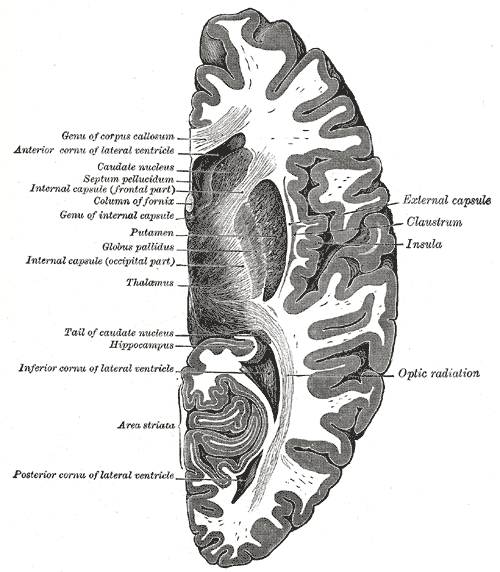
\includegraphics[height=0.5\linewidth]{thalamus}
	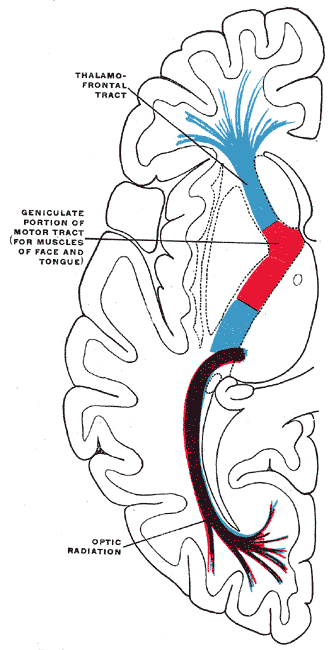
\includegraphics[height=0.5\linewidth]{frontalcortexfibers}
	\caption{The Thalamus, the Internal Capsule and fibers.  We wish to characterize the fibers which originate in the thalamus, pass through the internal capsule and end in the frontal cortex.  This image is from a diagram in Gray's Anatomy}
\end{figure}
The fibers that connect the thalamus and the frontal cortex are believed to be involved in the formation of memories.  Since Schizophrenia patients have difficulty forming and organizing memory, difficiencies in these fibers may explain these symptoms.  Additionally these fibers are interesting from a tractography standpoint because there are many other fibers which cross this set of fibers on their way to the frontal cortex.  In this regions of crossing, the diffusion is averaged with the crossing fiber resulting in a diffusion profile with reduced anisotropy.  This is precisely the situation for which stochastic tractography can be useful since streamlining methods would terminate in regions of low anisotropy possibly never reaching the frontal cortex.  So far, most studies of these fibers have been either per voxel analysis or streamlining tractography.  In this project, we study these fibers using our stochastic tractography method and compare our results with prior studies.

%show where the labels are using picture
\section{Method}
We performed the analysis on a total of 10 subjects, half diagnosed with schizophrenia, the other half are normal.  In each subject the right and left internal capsule were segmented by an expert.  Additionally a plane was labeled anterior to the internal capsule in the prefrontal cortex.  This plane was used to determine whether a fiber tract progressed towards the frontal cortex.

For each subject, an image of only the brain was extracted from the B0 image using FSL's BET tool.  This extracted image was then used as input to FSL's FAST algorithm to obtain a posterior probability for each voxel being white matter.

For every subject, stochastic tractgraphy algorithm generated 3000 sample tracts for every voxel in the right and left internal capsules.  Tracts which did not pass through the prefrontal labeled plane were discarded leaving tracts which progressed from the internal capsule to the frontal cortex.

\section{Results}

%include with and without white matter posterior probability map

%analysis of SNR

\subsection{Convergence of Statistics}
%show graphs of convergence
%Need to determine how to do this
\section{Discussion}
